\documentclass{article}
\usepackage{tabularx}
\usepackage{graphicx}
\usepackage{dirtytalk}
\usepackage{pgfplotstable} 
\usepackage{pgfplots}
\usepackage{datatool}
\usepackage{siunitx}
\usepackage[hyphens]{url}
\usepackage{hyperref}
\usepackage{graphicx}
\usepackage{microtype}
\usepackage{float}
\usepackage[style=ieee]{biblatex}
\usepackage{listings}
\usepackage{xcolor}
\usepackage[normalem]{ulem}
\usepackage{dirtytalk}

\definecolor{mygreen}{rgb}{0,0.6,0}
\definecolor{mygray}{rgb}{0.5,0.5,0.5}
\definecolor{mymauve}{rgb}{0.58,0,0.82}

\lstset{
    language=Java,                % Set language to Java
    basicstyle=\ttfamily\footnotesize, % Set font style and size
    keywordstyle=\color{blue},    % Set color for keywords
    stringstyle=\color{mymauve},  % Set color for strings
    commentstyle=\color{mygreen}, % Set color for comments
    numbers=left,                 % Line numbers on the left
    numberstyle=\tiny\color{mygray}, % Style for line numbers
    stepnumber=1,                 % Line number step size
    numbersep=10pt,               % Line number separation
    backgroundcolor=\color{white},% Background color
    showspaces=false,             % Do not show spaces
    showstringspaces=false,       % Do not underline spaces in strings
    showtabs=false,               % Do not show tabs
    frame=single,                 % Draw a frame around the code
    tabsize=4,                    % Set tab size
    captionpos=b,                 % Caption position (bottom)
    breaklines=true,              % Allow line breaking
    breakatwhitespace=false,      % Line breaks only at whitespace
    title=\lstname                % Show the filename of the code
}

\lstdefinestyle{bash}{
    language=bash,                % Set language to Bash
    basicstyle=\ttfamily\footnotesize, % Set font style and size
    keywordstyle=\color{blue},    % Set color for keywords
    stringstyle=\color{mymauve},  % Set color for strings
    commentstyle=\color{mygreen}, % Set color for comments
    numbers=left,                 % Line numbers on the left
    numberstyle=\tiny\color{mygray}, % Style for line numbers
    stepnumber=1,                 % Line number step size
    numbersep=10pt,               % Line number separation
    backgroundcolor=\color{white},% Background color
    showspaces=false,             % Do not show spaces
    showstringspaces=false,       % Do not underline spaces in strings
    showtabs=false,               % Do not show tabs
    frame=single,                 % Draw a frame around the code
    tabsize=4,                    % Set tab size
    captionpos=b,                 % Caption position (bottom)
    breaklines=true,              % Allow line breaking
    breakatwhitespace=false,      % Line breaks only at whitespace
    title=\lstname                % Show the filename of the code
}

\addbibresource{main.bib}

\hypersetup{
    colorlinks=true,
    linkcolor=blue,
    filecolor=blue,      
    urlcolor=blue,
    citecolor=blue,
}

\pgfplotsset{compat=1.18}

\title{\textbf{Lab 3 - Linearizability of Lock-free Skiplists\\Parallel and Distributed Computing\\DD2443 - Pardis24}}
\author{Names:\\Casper Kristiansson\\Nicole Wijkman\\\\Group 14}
\date{\today}

\begin{document}

\setlength\parindent{0pt}
\setlength{\parskip}{\bigskipamount}

\maketitle

\newpage
\section{Measuring Execution Time}

\subsection{Measurement program \& Dardel experiments}

\subsubsection{Explanation}
The execution time of the \texttt{LockFreeSkipList} was measured using a custom program with thread counts of 1, 2, 4, and 8. The operations were split into two mixtures: 10\% add, 10\% remove, and 80\% contains (1:1:8), and 50\% add and 50\% remove (1:1:0). The values were sampled from both normal and uniform distributions. Each thread executed 100,000 operations with 5 warmup rounds and 10 measurement rounds for final statistics.

The program was also run on Dardel (PDC) using thread counts up to 96. The same mixtures and distributions were applied, simulating larger workloads to observe scaling performance under higher contention.

\subsubsection{Results and Plots}

The following figures show the performance of the LockFreeSkipList with both normal and uniform distributions, across a range of thread counts.

\begin{figure}[H]
    \centering
    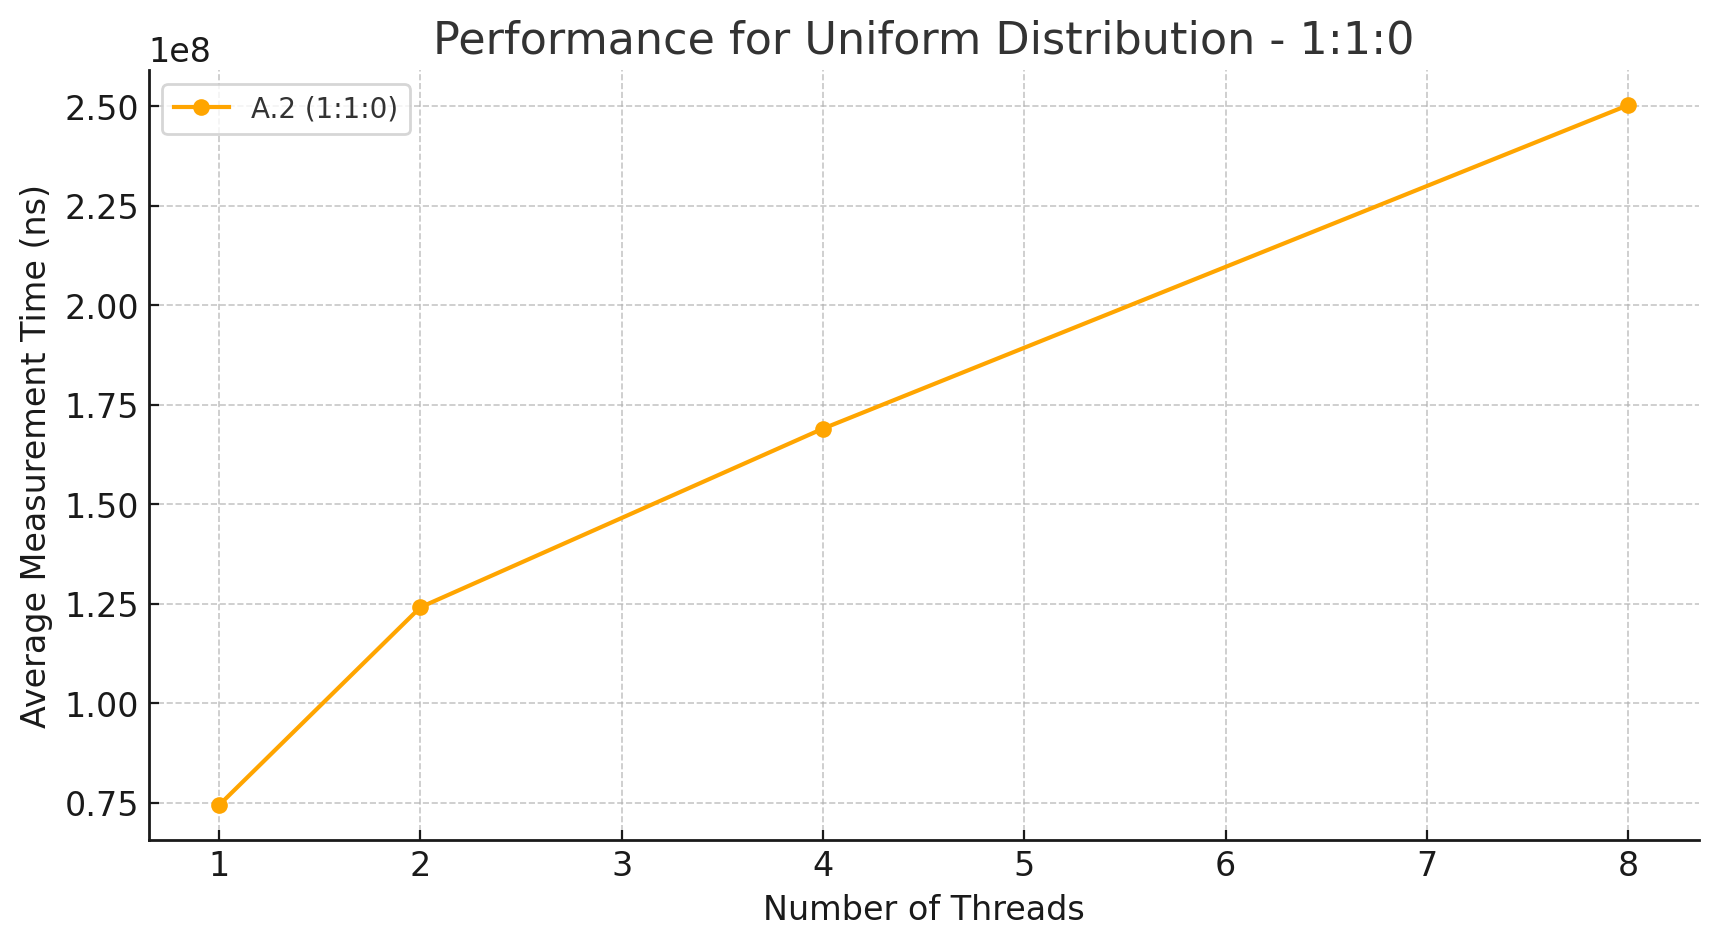
\includegraphics[width=\textwidth]{LaTex/images/Lab 3 1.2.1.png}
    \caption{Performance for Uniform Distribution - 1:1:0}
    \label{fig:enter-label}
\end{figure}

\begin{figure}[H]
    \centering
    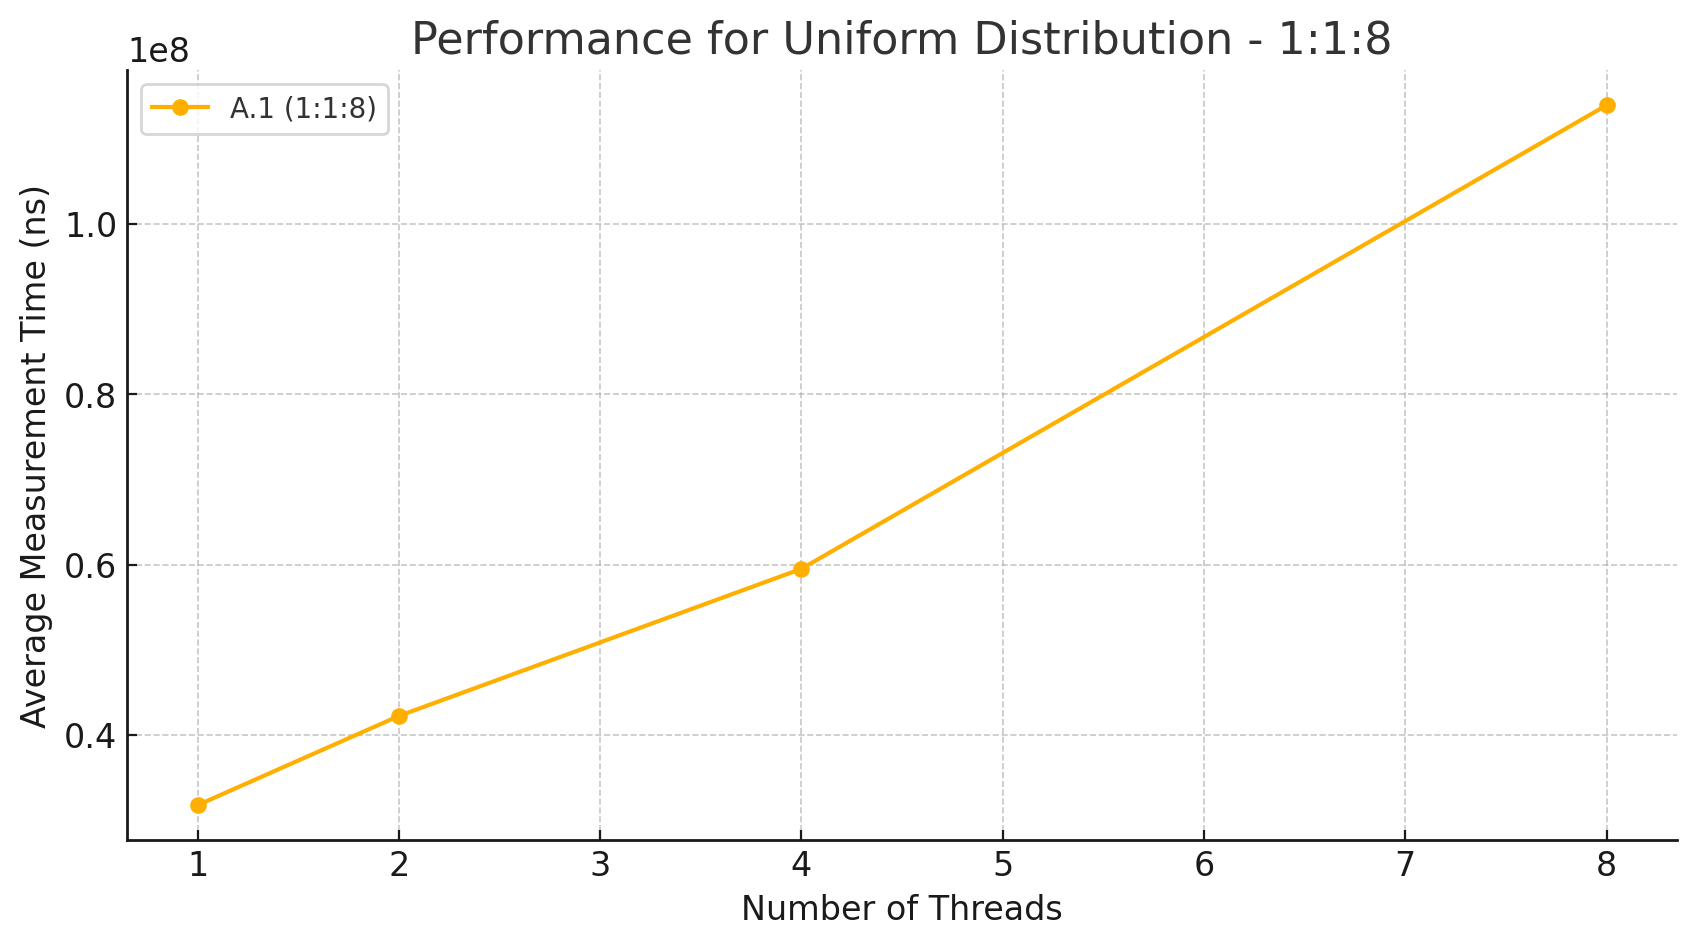
\includegraphics[width=\textwidth]{LaTex/images/Lab 3 1.2.2.png}
    \caption{Performance for Uniform Distribution - 1:1:8}
    \label{fig:enter-label}
\end{figure}

\begin{figure}[H]
    \centering
    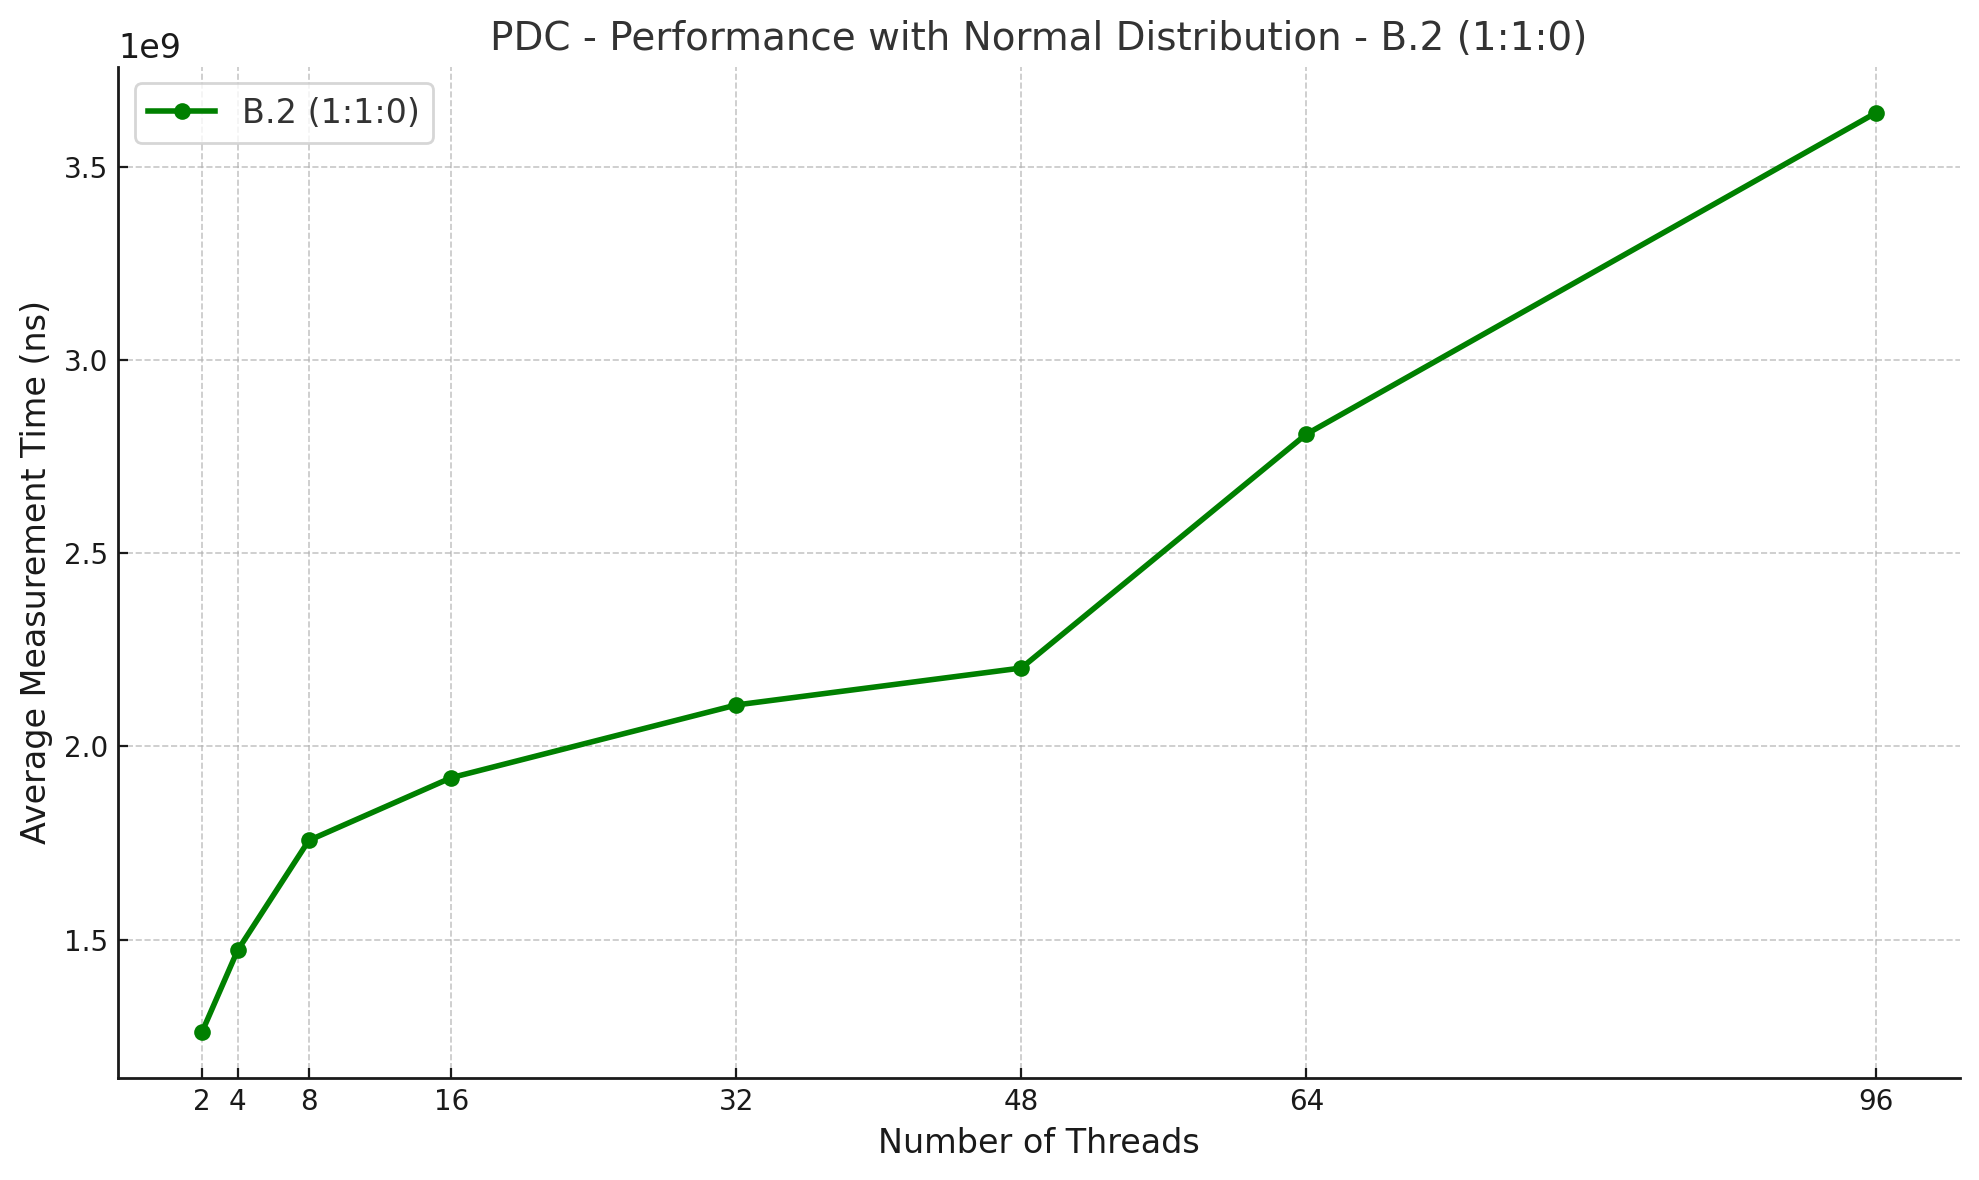
\includegraphics[width=\textwidth]{LaTex/images/Lab 3 1.2.3.png}
    \caption{PDC - Performance for Normal Distribution - 1:1:0}
    \label{fig:enter-label}
\end{figure}

\begin{figure}[H]
    \centering
    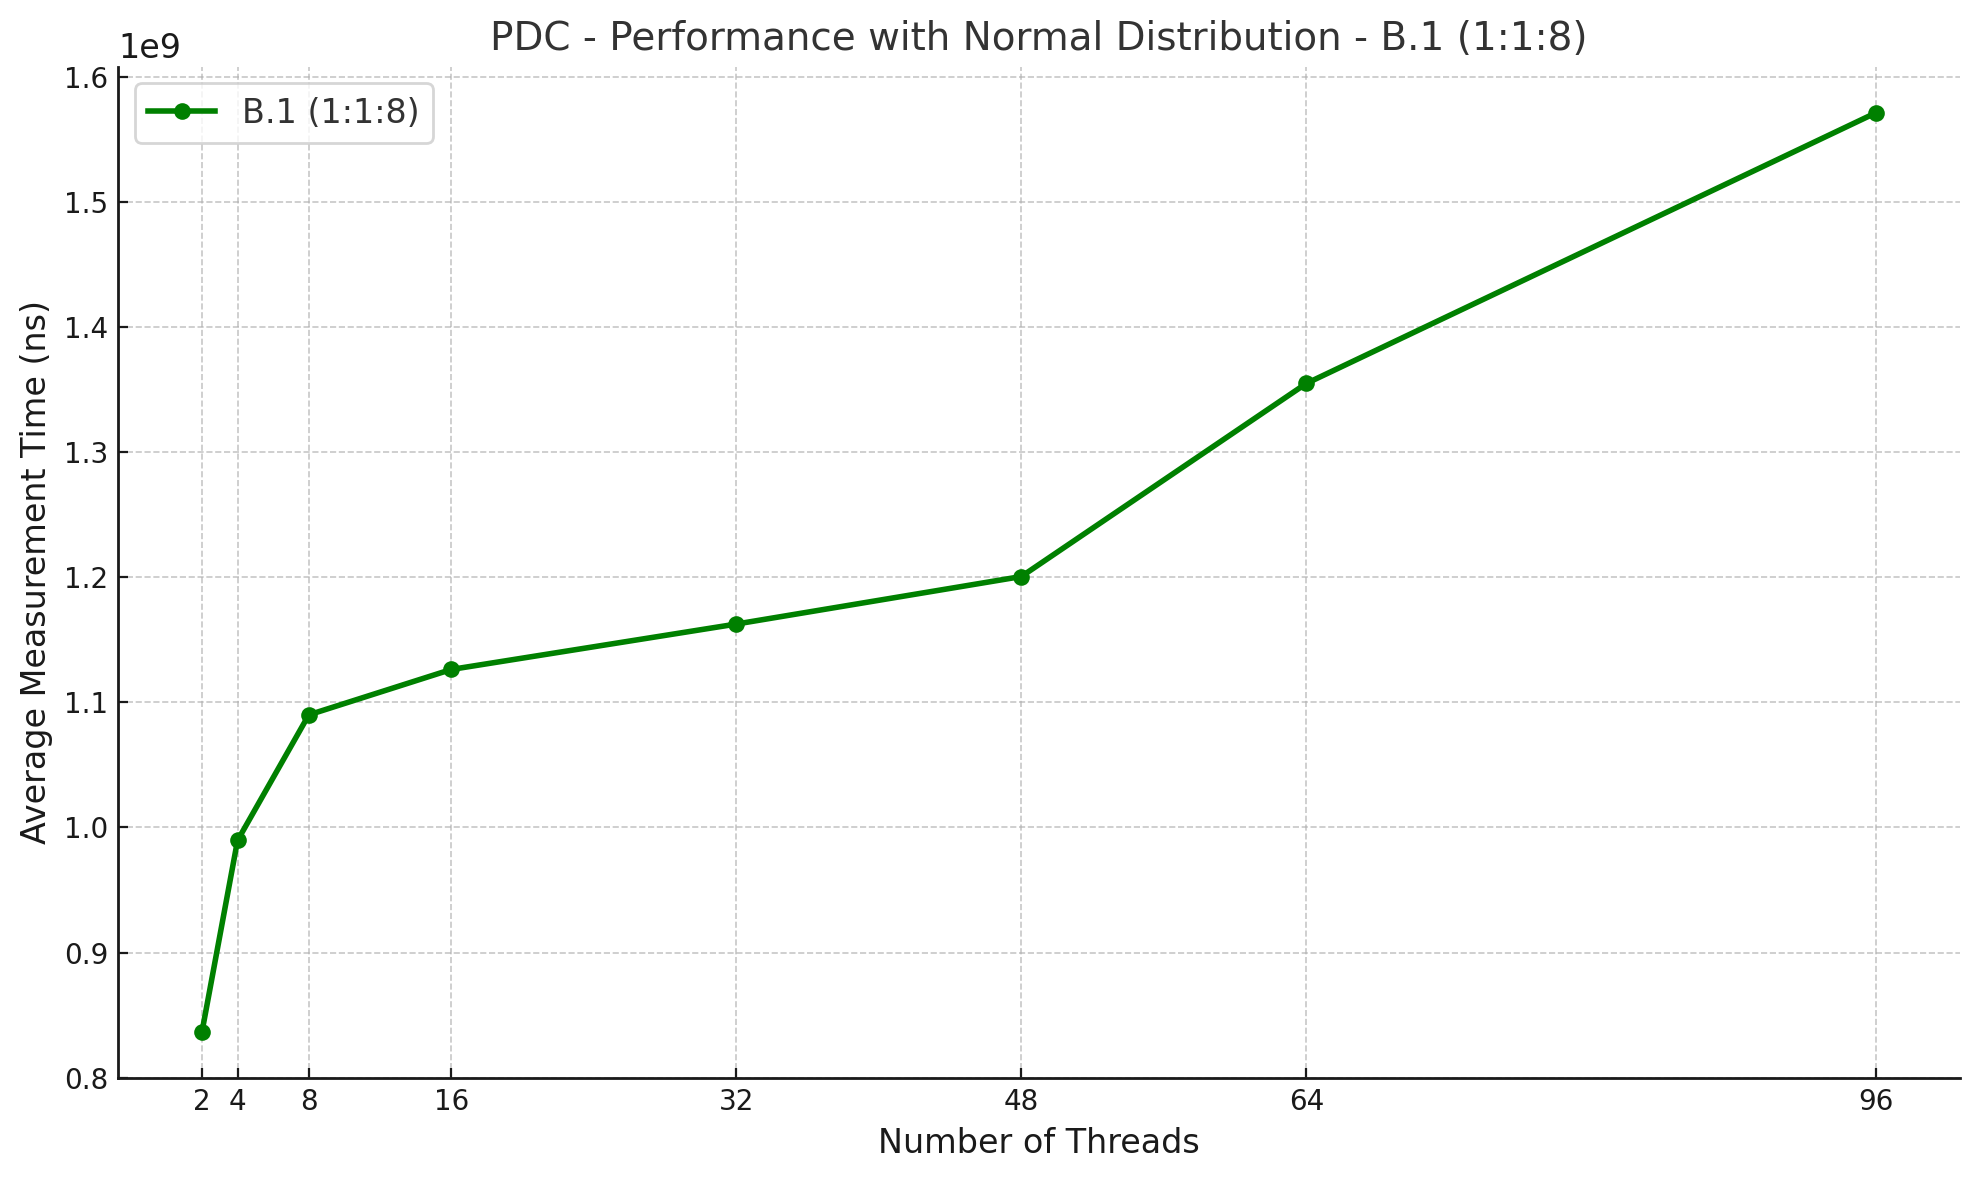
\includegraphics[width=\textwidth]{LaTex/images/Lab 3 1.2.4.png}
    \caption{PDC - Performance for Normal Distribution - 1:1:8}
    \label{fig:enter-label}
\end{figure}

\subsubsection{Discussion}
The results indicate that execution time increases with the number of threads, especially beyond 4 threads. This pattern holds across both the normal and uniform distributions and both operation mixtures. The initial decrease in execution time with up to 4 threads is due to improved parallelism. However, the overhead of managing higher thread counts causes the execution time to rise again with 8 threads.

In the Dardel experiments (Figures 3 and 4), the trends observed in local measurements are confirmed. As the number of threads increases up to 96, the performance degradation becomes more apparent, particularly for the 1:1:0 mixture. The read-heavy mixture (1:1:8) initially scales better, but with high thread counts, contention on shared resources becomes the limiting factor, leading to slower execution times.

The increased execution time with more threads is especially pronounced in the normal distribution cases (Figures 3 and 4). This is likely due to the distribution characteristics, where normal distribution results in a higher concentration of operations around the mean, increasing contention on certain key ranges.


\newpage
\section{Identifying and Validating Linearization Points}

\subsection{Identify Linearization Points}

\subsubsection{Explanation}
In the \texttt{LockFreeSkipList}, linearization points are the moments when operations appear to take effect atomically. These points ensure correctness in a concurrent environment.

For the \texttt{add()} method, the linearization point occurs when the \texttt{compareAndSet()} succeeds on the bottom-level reference, linking the new node into the list. If the node is already present, the linearization point is during the \texttt{find()} operation that detects the node’s presence.

In the \texttt{remove()} method, the linearization point of \texttt{remove()} occurs when a successful \texttt{compareAndSet()} marks the bottom-level node for removal (line 96 in the source code). For unsuccessful removals, the \texttt{find()} method is not the linearization point itself; rather, it helps in identifying the linearization point by determining whether a node has been logically removed (marked) in combination with other operations like \texttt{compareAndSet()}.

The \texttt{contains()} method’s linearization point happens when it checks the bottom-level list and observes whether the target node is unmarked. Success occurs when the target key is found, and failure when the key is missing.


\subsubsection{Discussion}
The linearization points for \texttt{add()}, \texttt{remove()}, and \texttt{contains()} are all based on atomic \texttt{compareAndSet()} operations, ensuring consistency across threads. In \texttt{add()} and \texttt{remove()}, it’s crucial to manage concurrent attempts to modify the same node, while \texttt{contains()} ensures it reflects the correct presence of the node. By placing linearization points at key \texttt{compareAndSet()} operations, we maintain the appearance of atomicity, which is vital for ensuring correct and efficient concurrent behavior.



\newpage
\subsection{Developing a Validation Method}

\subsubsection{Explanation}
The \texttt{LogEntry} class was designed to capture the linearization points by recording the method name (for example: \texttt{add()}, \texttt{remove()}, or \texttt{contains()}), the arguments (the hash code of the element), the return value (e.g., success or failure), and the exact timestamp using \texttt{System.nanoTime()}. For validation, the \texttt{Log.validate} method replays the log entries on a \texttt{HashSet} and compares the results. If the \texttt{add()} method returns true in the log but the \texttt{HashSet} shows it as false, this counts as a discrepancy. The number of discrepancies indicates the consistency of the log.

\subsubsection{Discussion}
The validation method worked effectively for capturing the linearization points for the \texttt{add()} and \texttt{remove()} operations, resulting in a low discrepancy count. The challenge was ensuring that the \texttt{contains()} method properly captures linearization points, as this operation only checks for the existence of an element and does not modify the skiplist, making it harder to validate with the same accuracy as \texttt{add()} and \texttt{remove()}. However, the overall log validation showed consistent and reliable behavior.

\newpage
\subsection{Locked Time Sampling}

\subsubsection{Explanation}
The locked time sampling method employs a \texttt{ReentrantLock} to synchronize the linearization point and time sampling. The lock ensures that no other threads can interleave, thereby capturing an accurate timestamp. In the \texttt{remove()} method, after a successful \texttt{compareAndSet()}, the timestamp is captured with \texttt{System.nanoTime()}. This ensures atomicity between the linearization point and time sampling. The same pattern is followed in the \texttt{add()} and \texttt{contains()} methods, providing consistency in time capture across all operations.

\subsubsection{Results and Plots}

The following plots show the performance of the locked time sampling method under different operation mixtures, including the results from Dardel experiments. The x-axis represents the number of threads, and the y-axis represents the measurement time in nanoseconds.

\begin{figure}[H]
    \centering
    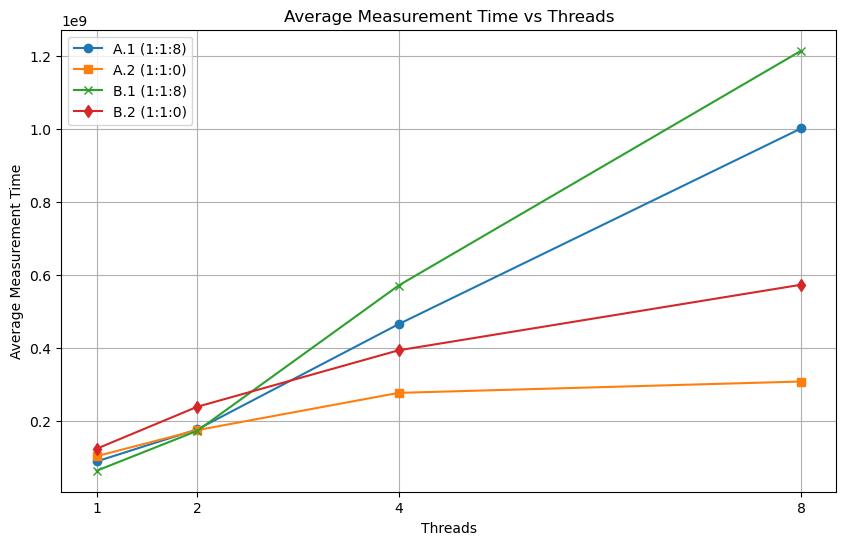
\includegraphics[width=\textwidth]{LaTex/images/Lab 3 2.3.2.1.png}
    \caption{Measurement Time vs Threads (A.1)}
    \label{fig:enter-label}
\end{figure}

\begin{figure}[H]
    \centering
    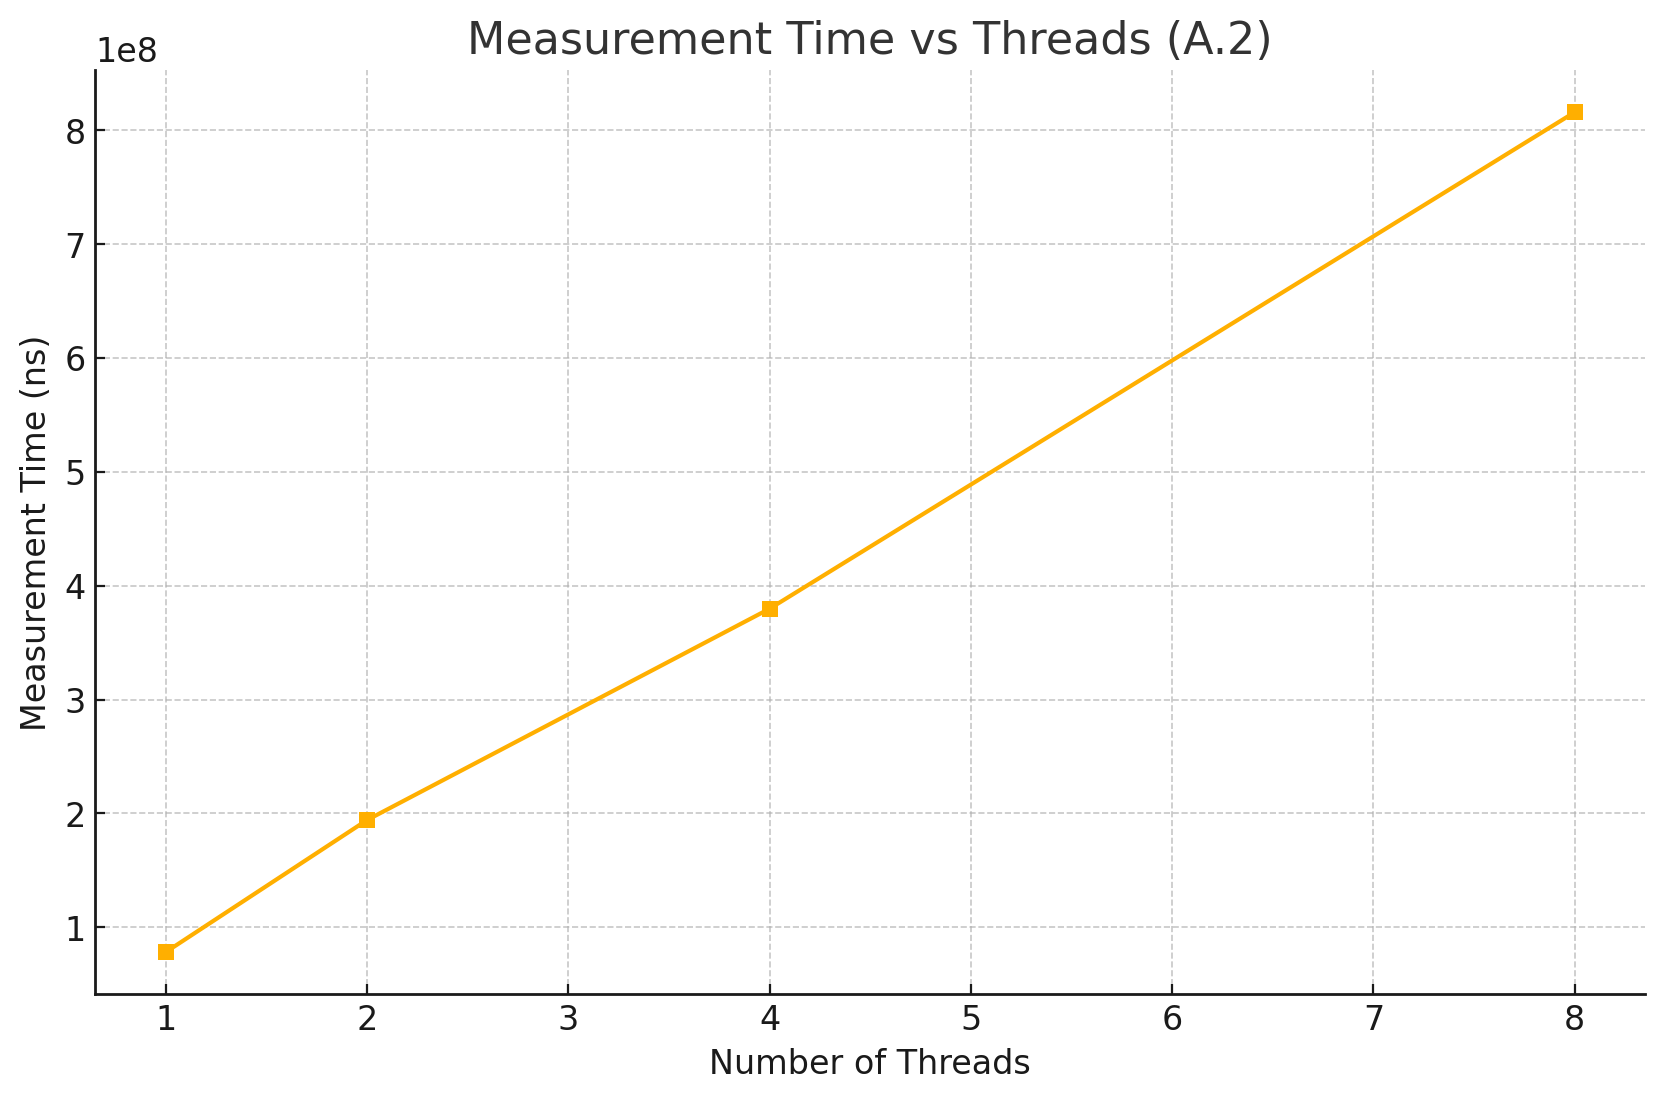
\includegraphics[width=\textwidth]{LaTex/images/Lab 3 2.3.2.2.png}
    \caption{Measurement Time vs Threads (A.2)}
    \label{fig:enter-label}
\end{figure}

\begin{figure}[H]
    \centering
    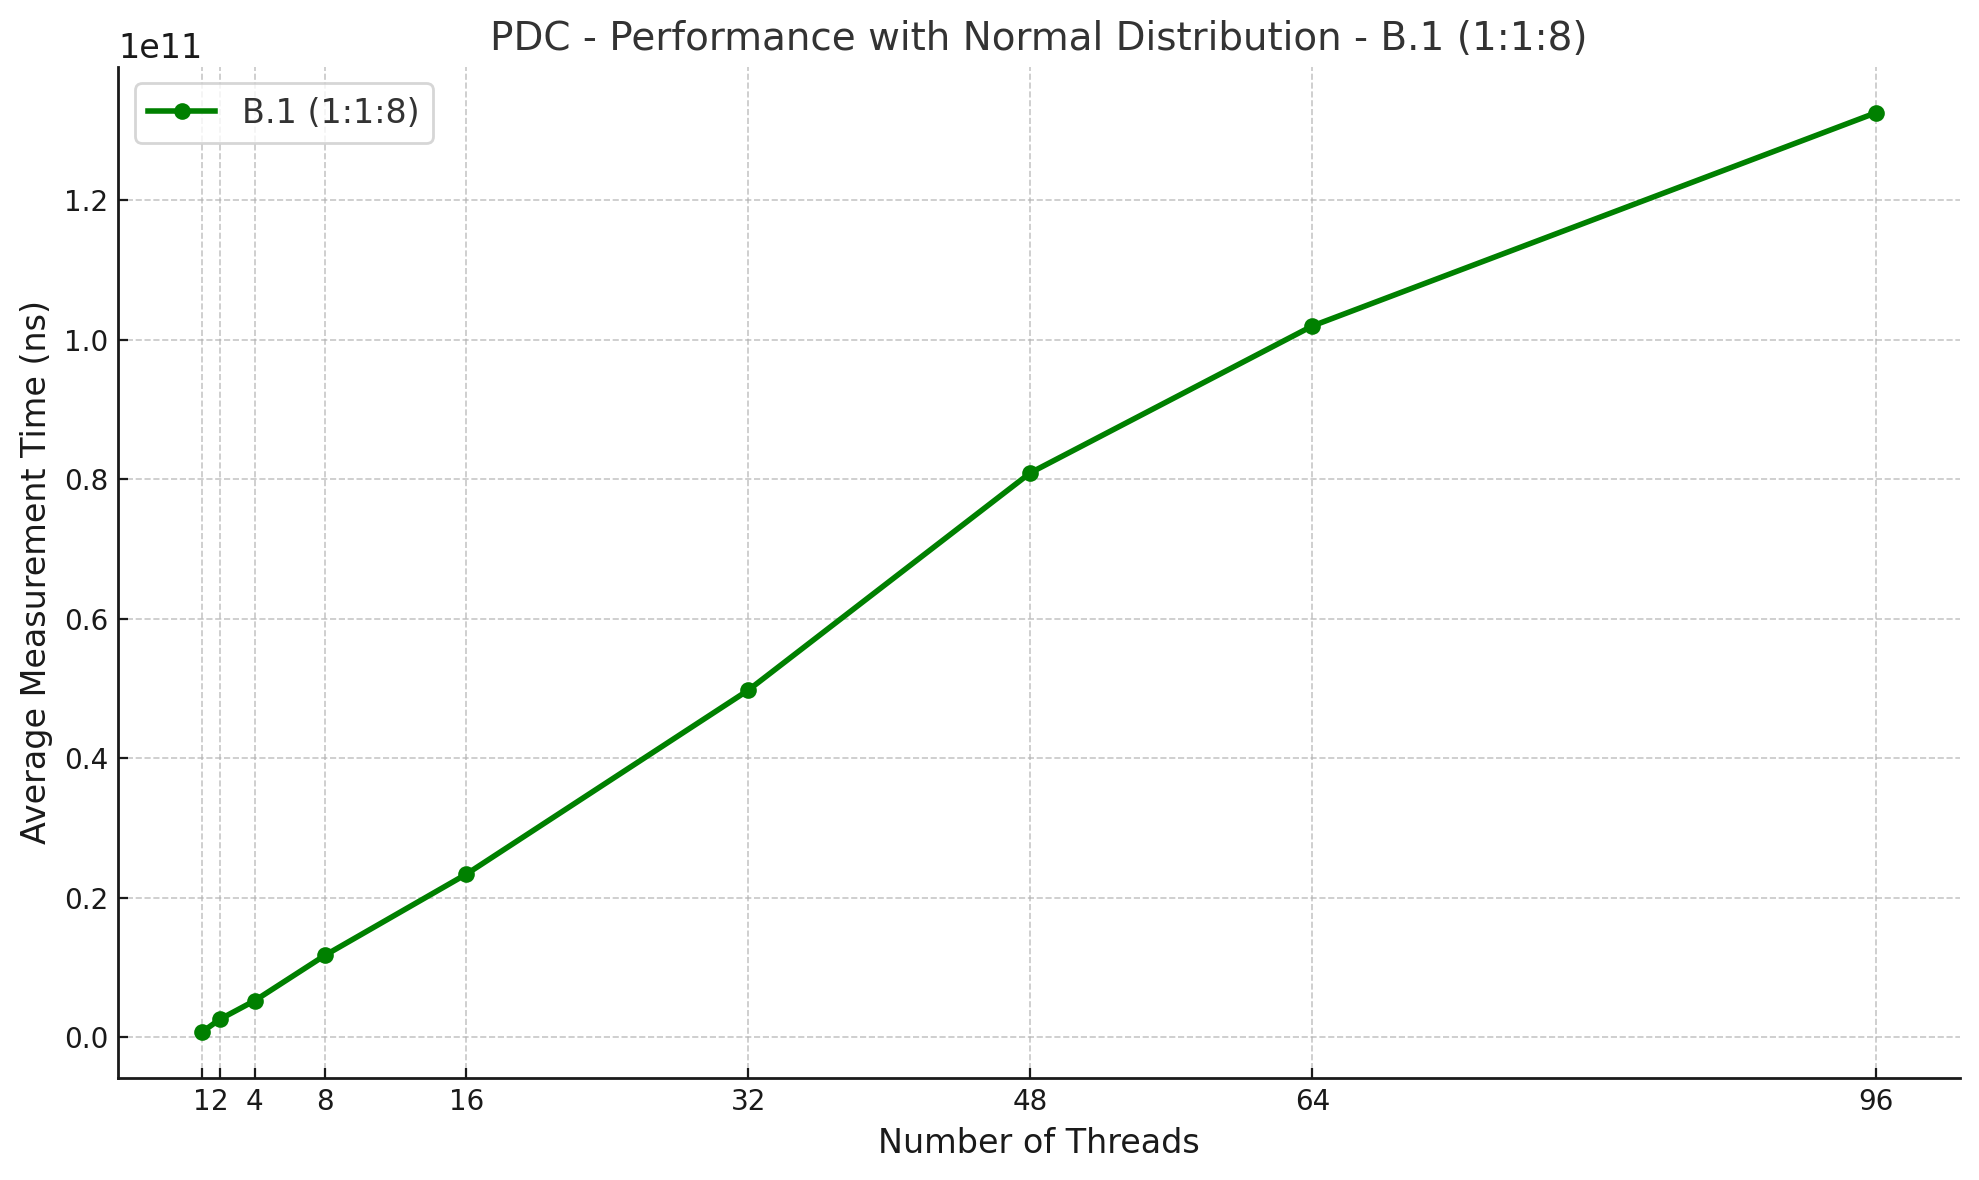
\includegraphics[width=\textwidth]{LaTex/images/Lab 3 2.3.2.3.png}
    \caption{Measurement Time vs Threads (B.1)}
    \label{fig:enter-label}
\end{figure}

\begin{figure}[H]
    \centering
    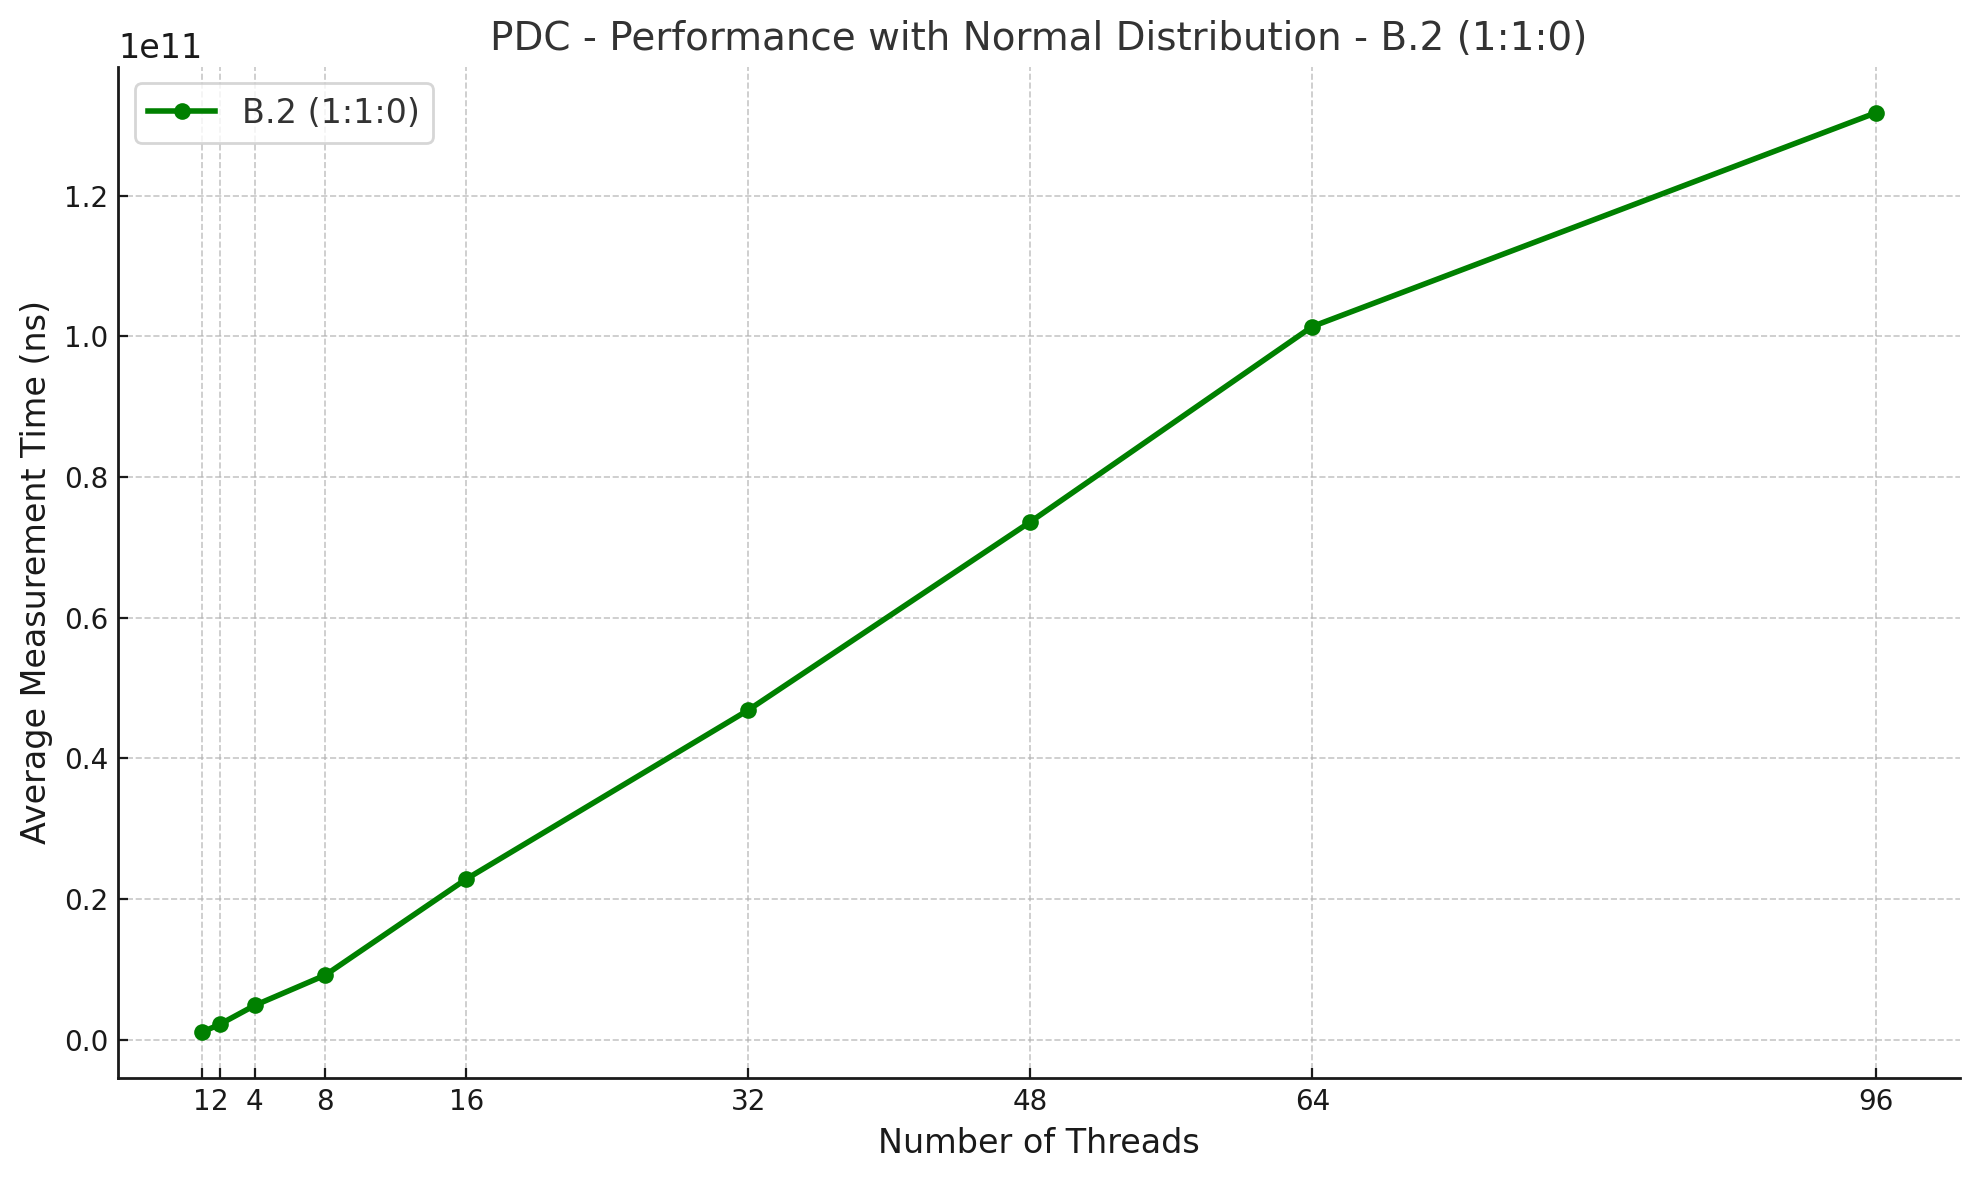
\includegraphics[width=\textwidth]{LaTex/images/Lab 3 2.3.2.4.png}
    \caption{Measurement Time vs Threads (B.2)}
    \label{fig:enter-label}
\end{figure}

\subsubsection{Discussion}
The locked time sampling method performed well in terms of accuracy, though it introduced minor latency due to the locking overhead. This was expected, as acquiring and releasing locks adds some delay. However, the use of locks ensured that time sampling and the linearization point were synchronized, resulting in minimal discrepancies.

In comparison to the local log method, the locked method provided more consistent and reliable measurements. The Dardel/PDC experiments further confirmed that the locked method maintained accuracy, even with higher thread counts, but at the cost of slightly increased measurement time. The results indicate that the method is more suited for scenarios where accuracy is critical, and synchronization costs are acceptable.

\newpage
\subsection{Lock-free Time Sampling with Local Log}

\subsubsection{Explanation}
In the lock-free time sampling method with local logs, each thread maintains its own local log, recording operations and time samples without any global lock. This reduces synchronization overhead and allows each thread to operate independently. At the end of the experiment, the local logs from each thread are merged into a global log and sorted by timestamp for validation. While this approach improves performance by avoiding global synchronization, it introduces the possibility of discrepancies due to interleaving between time sampling and the linearization point.

\subsubsection{Results and Plots}

The following plots show the performance of the lock-free time sampling method with local logs in different operation mixtures. The x-axis represents the number of threads, and the y-axis represents the measurement time in nanoseconds.


\begin{figure}[H]
    \centering
    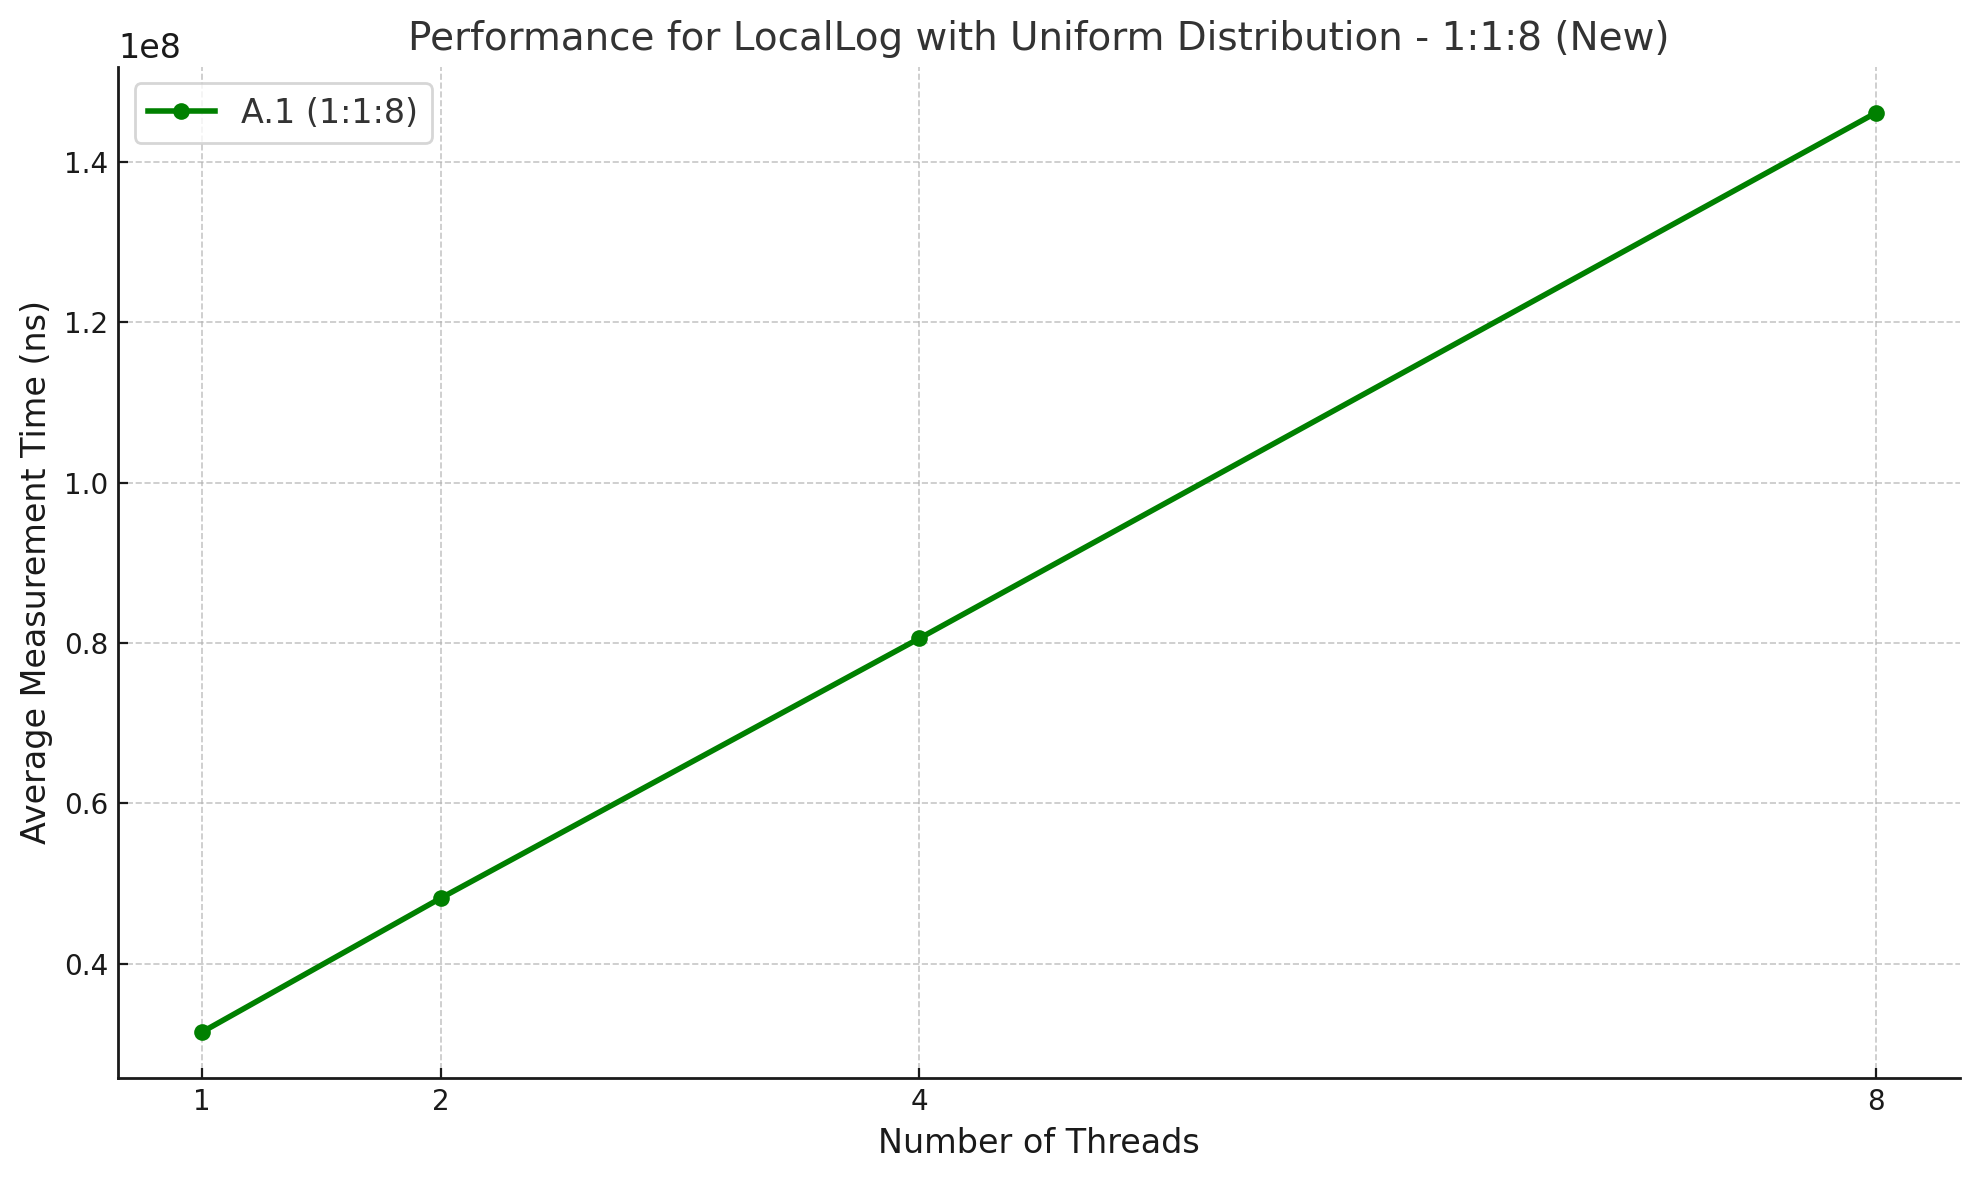
\includegraphics[width=0.9\textwidth]{LaTex/images/Lab 3 2.4.2.1.png}
    \caption{Performance for LocalLog with Uniform Distribution - 1:1:8}
    \label{fig:performance_a1}
\end{figure}

\begin{figure}[H]
    \centering
    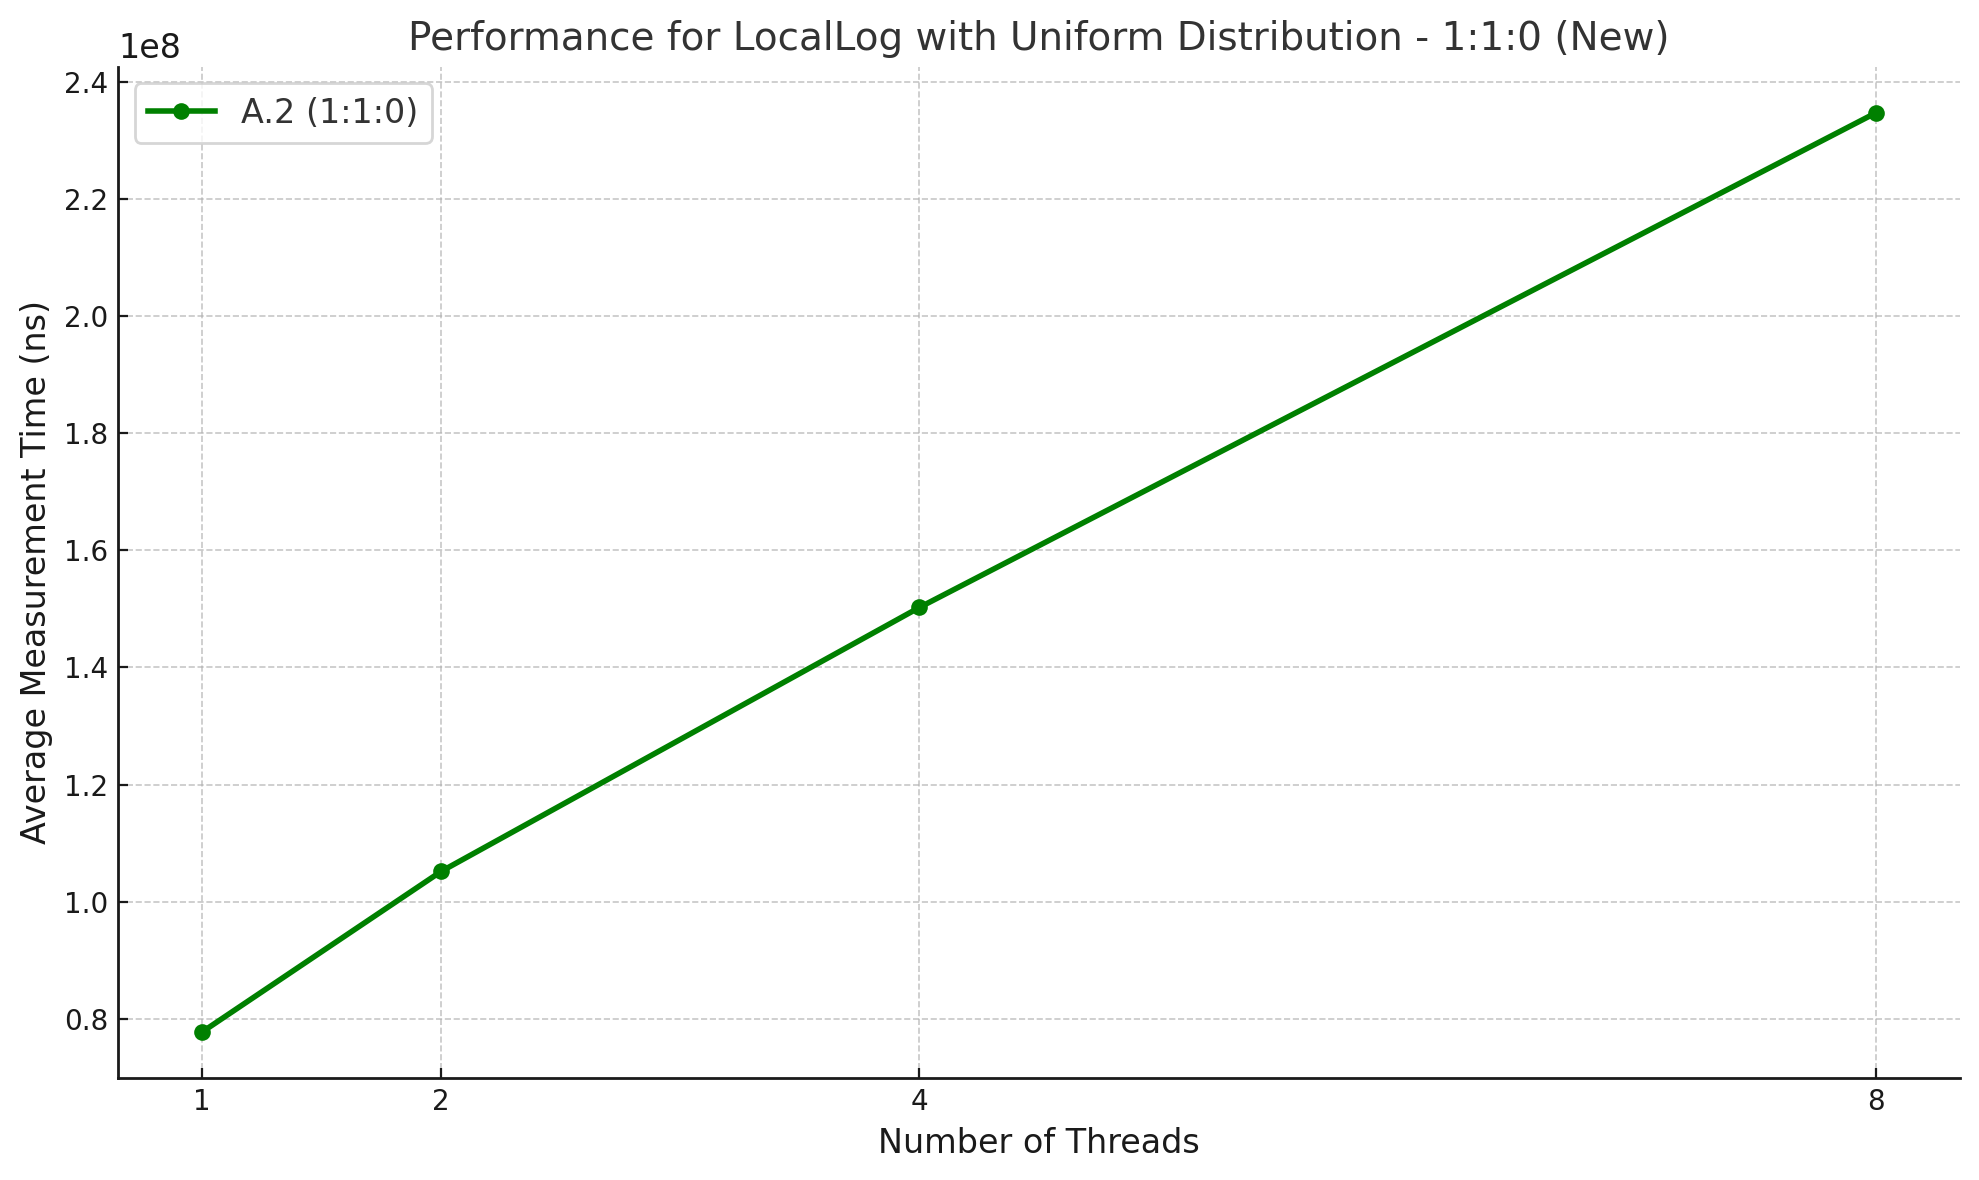
\includegraphics[width=0.9\textwidth]{LaTex/images/Lab 3 2.4.2.2.png}
    \caption{Performance for LocalLog with Uniform Distribution - 1:1:0}
    \label{fig:performance_a2}
\end{figure}

On Dardel, we measured both the execution time and the accuracy of the logs, using the same experimental cases from Task 1.2. The following plots show the execution time for the lock-free time sampling method with local logs under normal distribution scenarios.

\begin{figure}[H]
    \centering
    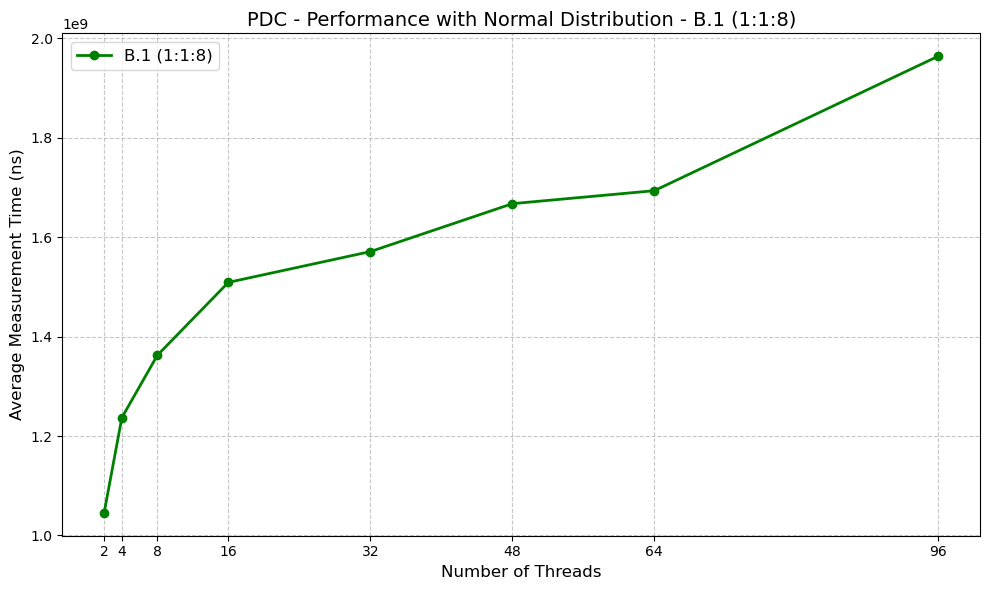
\includegraphics[width=0.9\textwidth]{LaTex/images/Lab 3 2.4.2.3.png}
    \caption{Performance for LocalLog with Uniform Distribution - 1:1:8 on Dardel}
    \label{fig:performance_dardel_1}
\end{figure}

\begin{figure}[H]
    \centering
    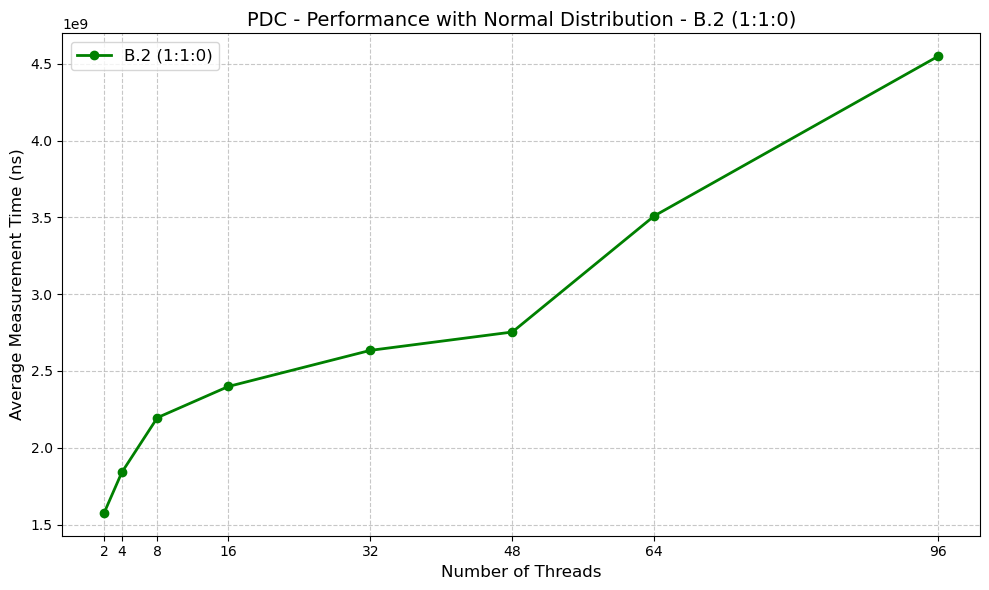
\includegraphics[width=0.9\textwidth]{LaTex/images/Lab 3 2.4.2.4.png}
    \caption{Performance for LocalLog with Uniform Distribution - 1:1:0 on Dardel}
    \label{fig:performance_dardel_2}
\end{figure}


\subsubsection{Discussion}
The lock-free local logging approach reduces overhead by eliminating global locks, improving performance, particularly with fewer threads. For thread counts of 1, 2, or 4, no discrepancies were observed, as fewer threads reduce the chance of interleaving between time sampling and linearization points. As the thread count increased to 8, minor discrepancies were detected, likely due to increased concurrency and the absence of global synchronization. However, the discrepancy count remained low, indicating that the method provides sufficient accuracy for workloads with moderate contention.

The Dardel experiments confirmed the scalability of the lock-free local logging method across a higher number of threads. As seen in Figures \ref{fig:performance_dardel_1} and \ref{fig:performance_dardel_2}, the execution time increased linearly as the number of threads increased, while accuracy remained consistent. This reinforces the suitability of the method for high-concurrency workloads with moderate synchronization requirements, while ensuring minimal discrepancies.


\newpage
\subsection{Lock-free Time Sampling with Global Log}

\subsubsection{Explanation}
The global lock-free time sampling method utilizes a concurrent lock-free queue from \texttt{java.util.concurrent}. Each thread writes directly to a global log with non-blocking operations, minimizing synchronization overhead. After all threads complete, log entries are sorted and validated. While this method improves scalability, it may introduce minor discrepancies due to interleaving between time sampling and linearization points.

\subsubsection{Results and Plots}
The following plots show the performance of the global lock-free time sampling method under different operation mixtures, along with Dardel experiments. The x-axis represents the number of threads, and the y-axis represents the measurement time in nanoseconds.

\begin{figure}[H]
    \centering
    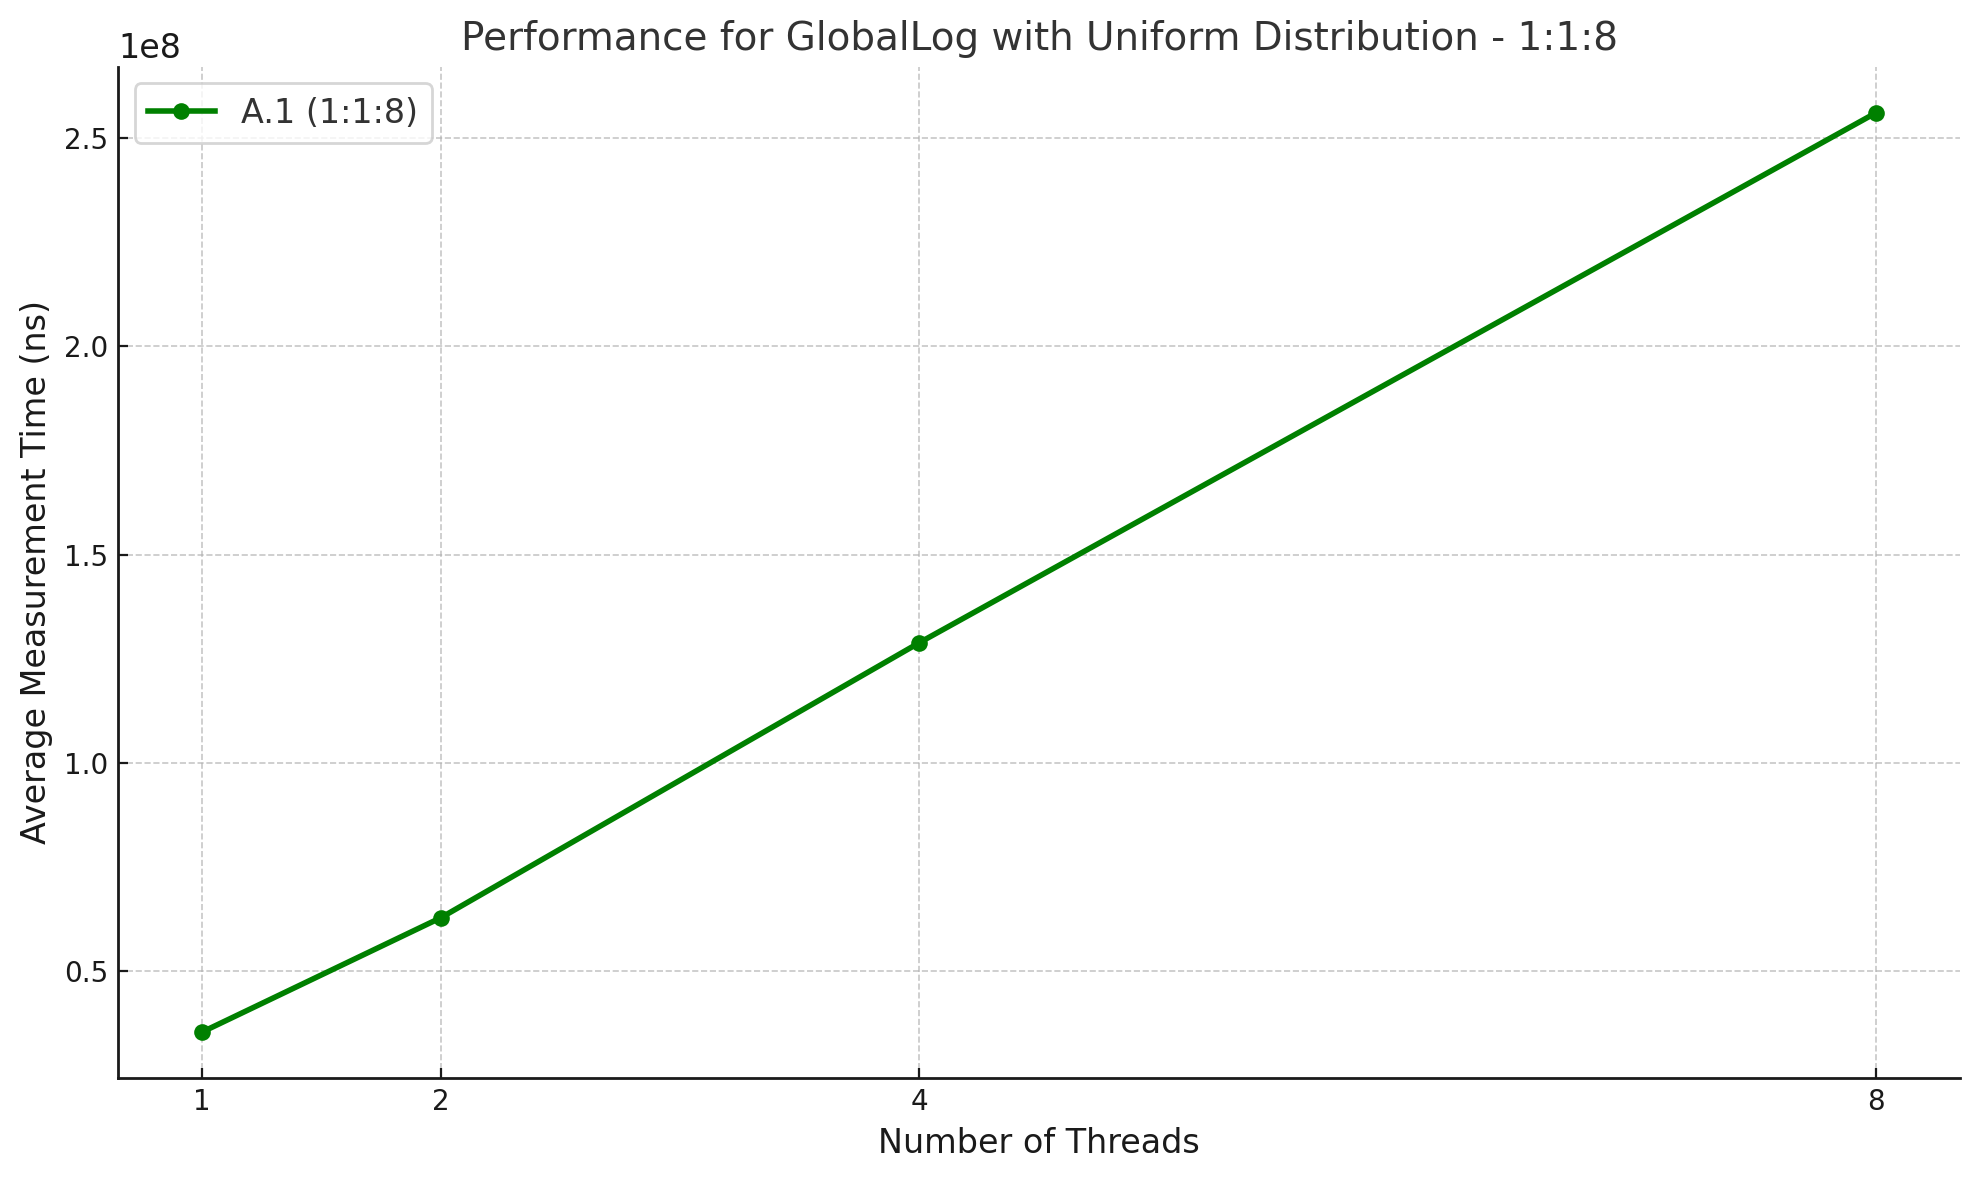
\includegraphics[width=\textwidth]{LaTex/images/Lab 3 2.5.2.1.png}
    \caption{Measurement Time vs Threads (A.1: 1:1:8)}
    \label{fig:global-log-1-1-8}
\end{figure}

\begin{figure}[H]
    \centering
    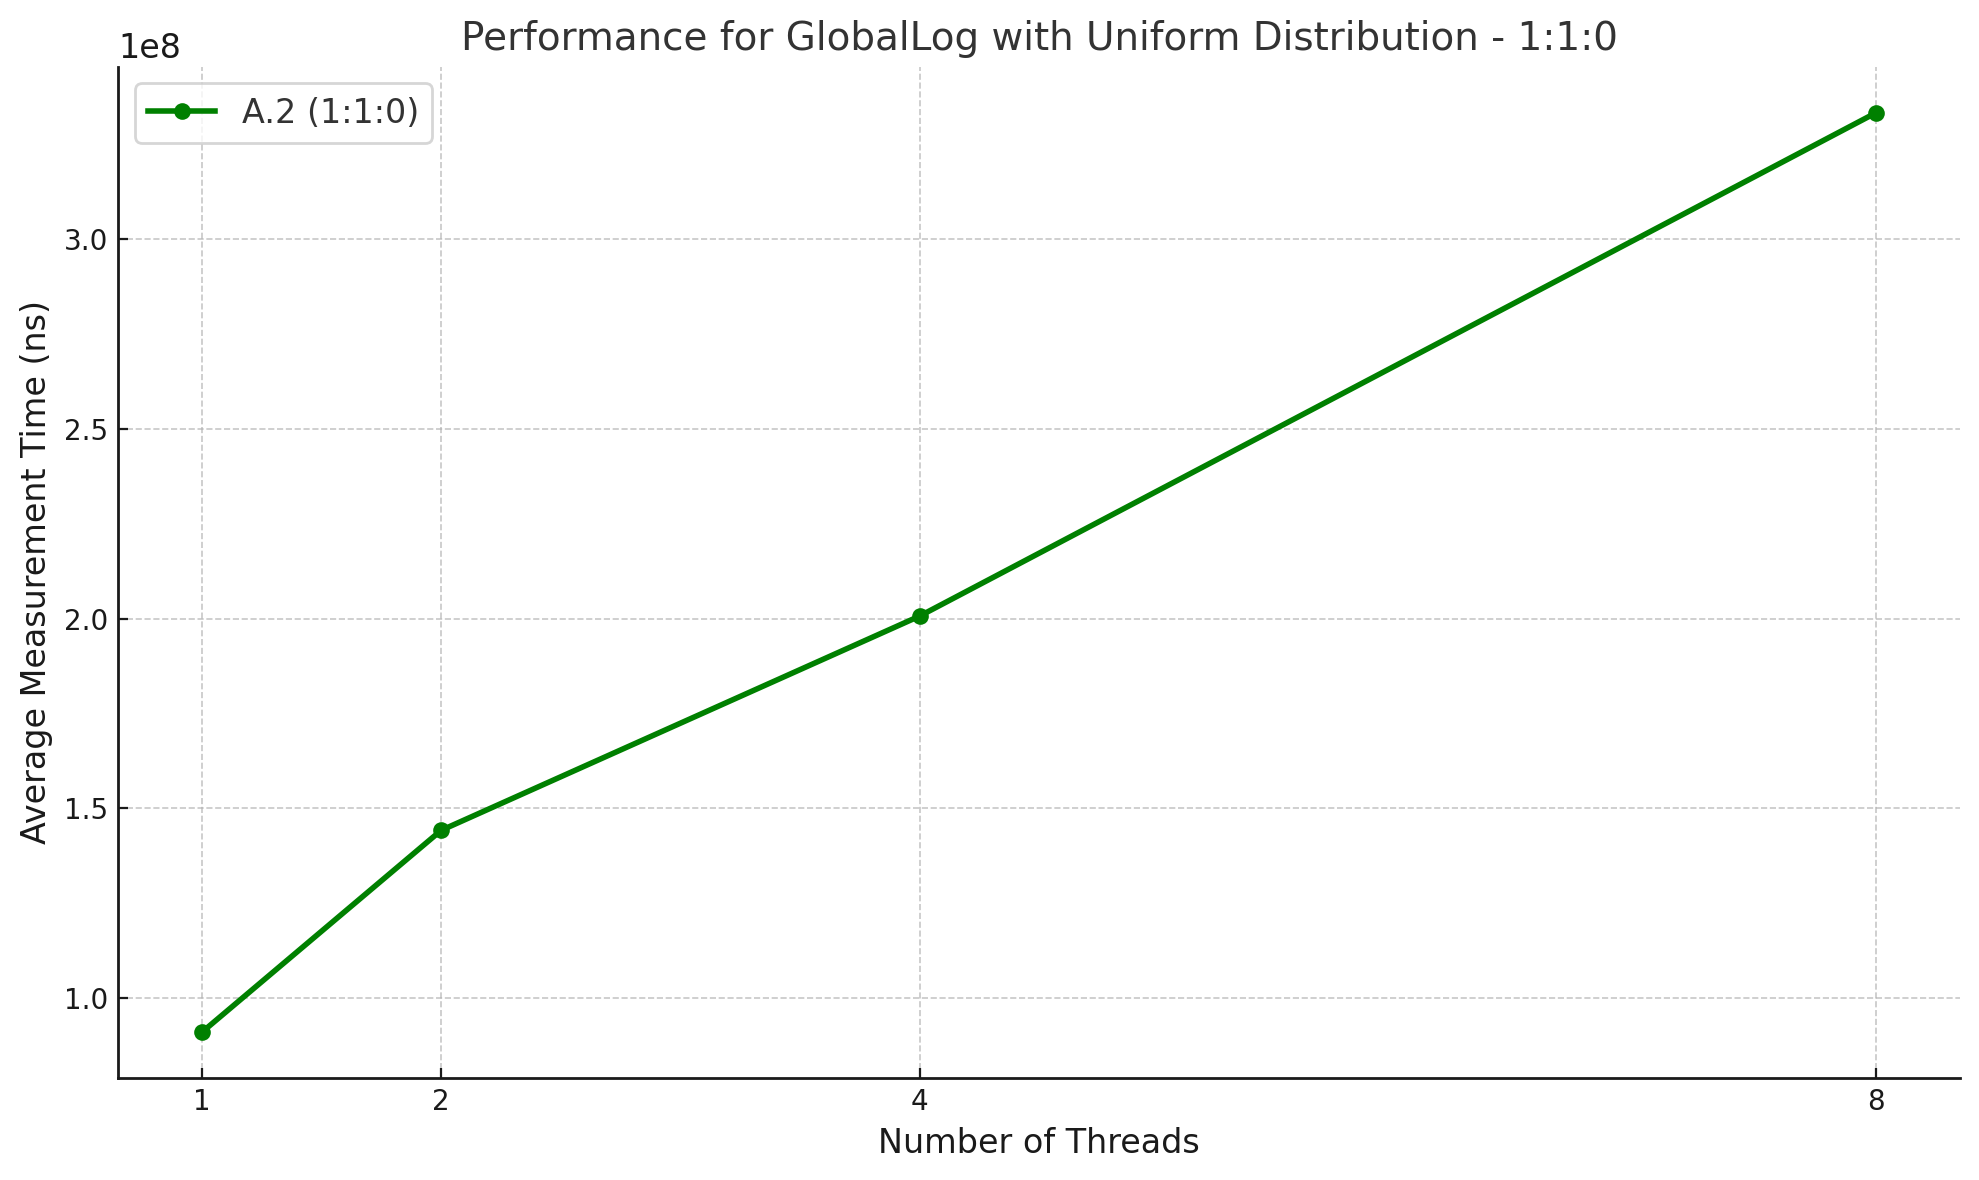
\includegraphics[width=\textwidth]{LaTex/images/Lab 3 2.5.2.2.png}
    \caption{Measurement Time vs Threads (A.2: 1:1:0)}
    \label{fig:global-log-1-1-0}
\end{figure}

\begin{figure}[H]
    \centering
    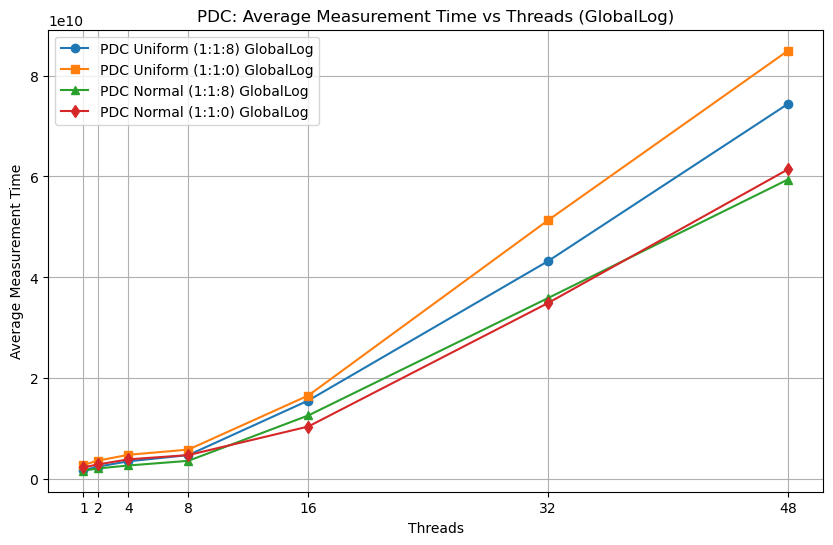
\includegraphics[width=\textwidth]{LaTex/images/Lab 3 2.5.2.3.png}
    \caption{Measurement Time vs Threads (B.1: 1:1:8) on Dardel}
    \label{fig:global-log-1-1-8}
\end{figure}

\begin{figure}[H]
    \centering
    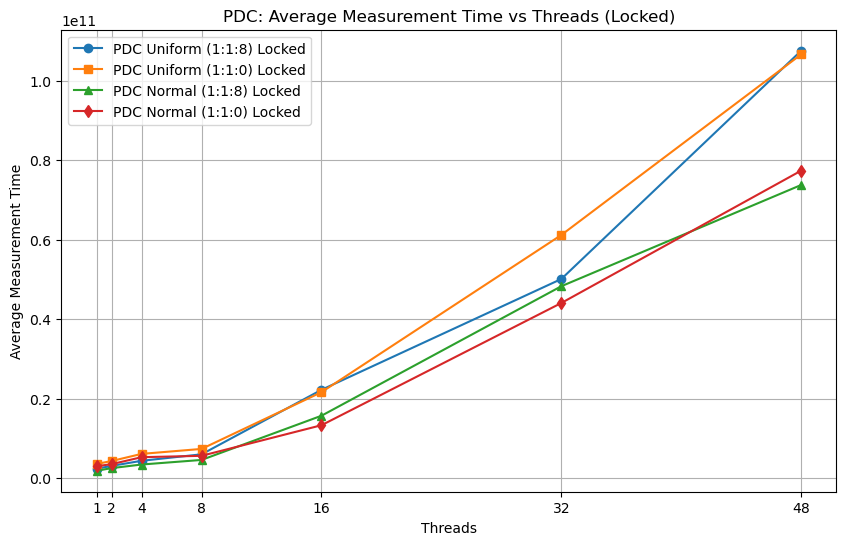
\includegraphics[width=\textwidth]{LaTex/images/Lab 3 2.5.2.4.png}
    \caption{Measurement Time vs Threads (B.2: 1:1:0) on Dardel}
    \label{fig:global-log-1-1-0}
\end{figure}

\subsubsection{Discussion}
The global log method demonstrated the best performance, particularly in scaling to higher thread counts, as seen in both the local and Dardel experiments. Minimal synchronization overhead resulted in a nearly linear increase in measurement time as the thread count increased.

While minor discrepancies were observed at 8 threads, these were caused by the interleaving of log entries rather than inaccuracies in \texttt{System.nanoTime()}. In the Dardel experiments, the method maintained high accuracy and efficiency, confirming its suitability for high-concurrency workloads where reducing synchronization is critical. The Dardel experiments also show that for larger thread counts, particularly with the B.1 and B.2 mixtures, the method continues to scale well, maintaining acceptable accuracy and performance even as the number of threads reaches up to 96.


\newpage
\printbibliography

\end{document}
